\section{Implementation}
The ETL engine and modules (extractions, transformations, loads) are implemented in JavaScript (\textit{ECMAScript 2017\textsuperscript{®}}) \cite{ecmascript2017} and designed to run in the context of the \textit{node.js} runtime environment \cite{nodejs}. \textit{node.js} emphasizes asynchronous input/output (IO), making it a good fit for handling ETL tasks in which IO (CouchDB is accessed exclusively via network requests) accounts for the greatest amount of computational overhead. Since \textit{node.js} runs server-side it provides access via JavaScript to the file system, which is required in terms of an ETL tool. JavaScript is a sensible language in which to implement nETL in the context of this project:

\begin{itemize}
    \item It has a very succinct API making it fast to write code in (i.e. it is a highly abstracted language similarly to Ruby or Python)
    \item But unlike Ruby or Python (and other high level languages), it is opinionated in that it handles IO asynchronously by default
    \item The JavaScript implementation of object-orientation is appealing (to some developers at least \cite{jsBook})
\end{itemize}

Modules are implemented via the \textit{revealing module} pattern, in which functions are returned from functions; parent functions create scoped execution environments that is similar in concept to instantiating classes\footnote{JavaScript has classes, but these are just syntactic sugar implemented partially via closure}. Compared to working with constructors closure provides more isolated scope. For each level of closure an additional scope is created that is available solely to functions defined within that scope. Figure \ref{fig-scope} shows code in which three scoped environments have been defined: a global scope, an Immediately Invoked Function Expression (IIFE) scope, and an \textit{exe}-function level scope (all of these are closed over by an \textit{invoke} function). JavaScript has \textit{lexical} scope \cite{jsBook2} that (for this purposes of this project) allows for configuring modules differently at different levels in object hierarchy without having to re instantiate modules that have already been loaded.

\begin{figure}[H]
  \centering
  \begin{mdframed}[rightline=true,leftline=true]
    \begin{minted}{text}
// Global scope

// Closure over the global scope
(function() {
    // Module-specific scope

    // Closure over module-specific scope
    function exe(configurationObj) {
        // Task-specific scope

        // Closure over task-specific scope
        function invoke() {...};

        return {
            invoke: invoke
        };
    };

    return {
        name: "MODULE_NAME",
        exe: exe
    };
})();
    \end{minted}
  \end{mdframed}
  \caption[Module Scope via closure]{\textbf{Figure \ref{fig-scope}: Scoping via closure in JavaScript}}
  \label{fig-scope}
\end{figure}

Modules are loaded into the nETL engine by invoking a function (an IIFE in terms of Figure \ref{fig-scope}) that returns an object with a \textit{name} property for identification and that references the \textit{exe} function. Loading many modules into the application results in a list of available module names, with each name in turn referencing a function named \textit{exe} (these are different functions with the same name). This is shown in Figure \ref{fig-module-memory} as the list with the heading \textit{Module Definitions}.

When a task specifies that a module should be used (identified by a name), A lookup for that name in the Module Definitions list is performed and the corresponding \textit{exe} function is executed. This returns a scoped execution context\cite{executionContext} in which another function called \textit{invoke} is required to be defined (nETL users author the body of the \textit{exe} function). The task assigns the name of the module to the \textit{invoke} function definition, which during task-execution may be called many times to perform extraction, transformation, or loading logic. A list of \textit{Loaded Modules} is maintained for each running task as shown in \ref{fig-module-memory}. Each of the referenced functions maintains closure over the execution context created on \textit{exe} invocation, thus allowing for a module to be loaded once but configured for specific tasks; every time an \textit{exe} function is called a new closed scope is created only accessible to the callee.

\begin{figure}[H]
    \centering
    \begin{mdframed}
        \centering
        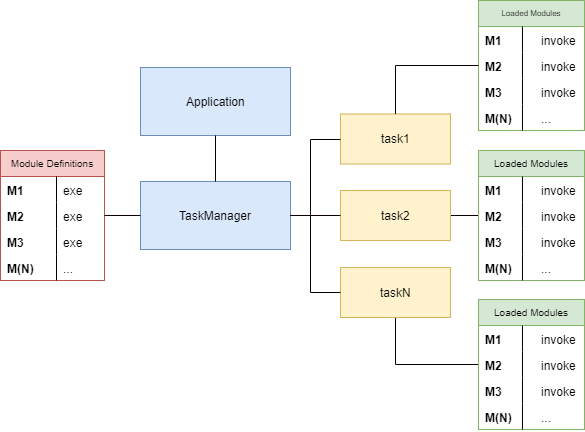
\includegraphics[scale=0.62]{./resources/figures/fig-module-memory.png}
    \end{mdframed}
    \caption[Loaded module representation]{\textbf{Figure \ref{fig-module-memory}: Loaded module representation}}
    \label{fig-module-memory}
\end{figure}

All modules adhere to the modular contract as shown in \ref{fig-module-contract} such that invoking a module returns a \textit{Promise} \cite{jsPromises} that resolves an \textit{invoke} function. This function accepts a single parameter and returns a \textit{Promise} that resolves the result of the module (which differs depending on whether a module performs extraction, transformation or loading operations). JavaScript \textit{Promise} objects are state-representation of asynchronous operations in terms of success and failure of these operations. Since logic implemented in a module may not be asynchronous, all logic is wrapped within a \mintinline{text}{setImmediate} function to ensure that the contract of asynchronous execution of all modules is adhered to (except for where generators are used, since \textit{ECMAScript 2017\textsuperscript{®}} does not support asynchronous generator functions).

\begin{figure}[H]
  \centering
  \begin{mdframed}
    \centering
    \begin{minted}{text}
(function () {
    // Execution context ('this') is a config object
    function invoke(obj) {
        return new Promise((resolve, reject) => {
            setImmediate(() => {
                try { resolve(obj); }
                catch (error) { reject(error); };
            });
        });
    };
    return new Promise(async(resolve, reject) => {
        setImmediate(() => {
            try { resolve({ invoke: invoke }); }
            catch (error) { reject(error); };
        });
    });
})();
        \end{minted}
  \end{mdframed}
  \caption[nETL module contract]{\textbf{Figure \ref{fig-module-contract}: nETL module contract}}
  \label{fig-module-contract}
\end{figure}

On task execution (as directed by a user via the CLI) a task is run from beginning to end, iteratively extracting batches of data from a source, transforming that data, loading that data and then repeating the process. Since IO in JavaScript is asynchronous, batching either needs to be run sequentially (batches are processed one after the other), or by carefully managing asynchronous execution of batches. Batches extracted asynchronously and concurrently would quickly overwhelm the network capabilities of any computer since thousands of network requests would be queued instantaneously (network IO is many times slower than file IO, which is many times slower than data transformation). Most of these requests would fail - it is easier to serialize processing of batches than to queue network requests. As such, nETL is implemented to execute separate tasks concurrently; but a single task comprises a series of sequential steps.

JavaScript is not truly parallel - concurrent execution is achieved via adding procedures to an event loop that is executed on a first-in first-out basis via a single thread, with certain operations specified to be implemented asynchronously. Certain functions in JavaScript (\mintinline{text}{setTimout}, \mintinline{text}{setImmediate}, and \mintinline{text}{setInterval}) along with certain environment-provided APIs (such as the node.js filesystem API) pass control back to the event loop before execution of these functions is completed. Such operations allow for specifying a callback function that is added to the event queue at time later from when the asyncrhonous function is first called. So if two tasks are running concurrently and a blocking procedure is called that is not asynchronous, processing of the event queue would be paused until the blocking procedure is completed. As a result, both tasks would be blocked until the procedure completes and the next item on the event loop is processed.

For this reason each step in the ETL engine (extraction, transformation and loading) is implemented asynchronously. Prior to the ECMAScript 2017 specification, an ETL engine implemented in node.js would have been challenging and require complex state management of asynchronous operations. But via the \textit{async}/\textit{await} API (a wrapper for JavaScript \textit{Promises}), such state management is straightforward as shown in Figure \ref{fig-engine} \footnote{Actually the extraction operation (\mintinline{text}{batch = batch.next()}) is NOT awaited (the \mintinline{text}{next} function is not asynchronous) because asynchronous generators are not supported in ECMAScript 2017}.

\begin{figure}[H]
  \centering
  \begin{mdframed}[rightline=true,leftline=true]
    \begin{minted}{text}
while (!batch.done) {
    values = batch.value;
    payload = await values.reduce(async(previousResults, item) => {
        const results = await previousResults;
        await asyncForEach(transformations, async(t) => {
            item = await t.invoke.call(t, item);
        });
        if (item !== {} && item) results.push(item);
        return results;
    }, []);
    loadResult = await load.invoke(payload);
    batch = batches.next();
};
    \end{minted}
  \end{mdframed}
  \caption[Serializing asynchronous operations]{\textbf{Figure \ref{fig-engine}: Loop with serialized asynchronous operations}}
  \label{fig-engine}
\end{figure}

\subsection{Extracting data}
Files are read in 64KB chunks from beginning to end within the context of an iterator created by a JavaScript \textit{generator} function \cite{mozillaGenerators}. Chunks are held in memory, split into lines (identified by \textit{LF}, \textit{CR} or \textit{CRLF} line ending markers to allow for cross-platform portability) and yielded a single line at a time to a controlling function executed within the context of the iterative ETL engine. This function iteratively collects \mintinline{text}{n} lines at a time into a list (\mintinline{text}{n} is a user configurable property \textit{batchSize}) and yields ``lists of lines'' - (\textit{batches}). Generators are useful in the regard because they automatically create a state handling mechanism for iterating over file contents - i.e. pointers to positions in files, references to incomplete lines as retrieved from files, etc. Disk access via generators is achieved via code taken directly from an open-source library \cite{bower16}.

Lines in batches are then transformed concurrently, with transformations (specified in configuration) applied to each line in the batch in the order specified in the configuration. Concurrent processing of items accessed via a loop is achieved by wrapping the loop body in an asynchronous function (\mintinline{text}{setImmediate}), allowing the loop to progress without waiting for loop body execution to complete.

The loop itself is awaited, however, and once all transformation have been applied to all lines in the batch (lines can also be discarded from the batch depending on the transformations applied), the transformed batch is returned to \mintinline{text}{taskManager} and passed as an argument to the loading function specified via configuration. The function's contract is such that \textit{taskManager} is notified when the batch has been loaded successfully to the destination, at which a further batch of lines is generated and processed. This batching loop is repeated until the extraction generator returns false when the end of a data source is reached.

\subsection{Transforming data}
In terms of processing lines in a flatfile (CSV format), headers are only ever read once with the assumption that the all rows can be split into values (by some defined delimiter) and that the order of the values corresponds with the order of the headers - if this is not the case, then the CSV is malformed. A reference to the CSV header row that is maintained for the duration of the transformation. CSV rows are iteratively loaded into memory and split into values. Row values are matched with header values to form key:value pairs and create JavaScript objects

After transforming row-strings into row-objects, additional transformations are applied to each object. The following transformations are applied to objects:

\begin{itemize}
    \item \textbf{Selection-filter:} Entire objects can be whitelisted based on properties and allowed values for those properties.
    \item \textbf{Join-selection-filter:} A list of attributes and values can be retrieved from a \nth{3} party data source (for example from a CouchDB index), and entire objects can be whitelisted based on the retrieved attributes and allowable values for those attributes. This is similar in concept to a join, although no means of actually joining documents is provided (i.e. creating attributes based on data retrieved from a \nth{3} party data source instead of applying selection - although this would be a fairly easy feature to implement).
    \item \textbf{Projection-filter:} Unneeded attributes can be removed from objects prior to loading into database/other destinations
    \item \textbf{Projection-append-attributes:} Additional attributes can be added to objects - e.g. a \textit{type\_} attribute can be added, along with a value as specified by configuration
\end{itemize}

\subsection{Loading data}
Batches of objects are serialized to JSON and are loaded into a CouchDB database via the the HTTP POST \_bulk\_docs endpoint (as opposed to separate network requests for each item in a batch). Bulk inserts are configured to be atomic - i.e. either an entire insert succeeds or fails. Network requests make use of the well-known, open-source node.js library ``request'' \cite{request-lib}.